\chapter{Introduction}
People have always been curious about new forms of visualization and illusion of reality. In the last decade computer generated imagery has reached a state, when majority of the public can't distinguish real photographs from entirely synthesized images. Thanks to this advancements we can enjoy otherwise impossible film shoots, imaginary worlds, visualizations of non existing buildings and much more. All this become possible, because ways how to represent objects and simulate light transport using computer algorithms have been found. The other important factor is ever growing computation power of these devices, which enables us visualize highly detailed datasets with complex materials and challenging lighting scenarios.
\\
\\
Even though many things are possible to simulate and visualize efficiently these days volumetric phenomenons such as clouds, smoke and other optically active medias are still real challenge even for high-end computers. This is all caused by the fact that the data we try to visualized are volumetric and that light passing through can be absorbed, scattered or even emitted in different wavelength (fig \ref{fig:AURO}). This means that we can no longer assume that visibility of an object can be determined simply by determining if it is hidden behind other object or not.
\\
\\
\begin{minipage}{\linewidth}
      \begin{minipage}{0.45\linewidth}
          \begin{figure}[H]
              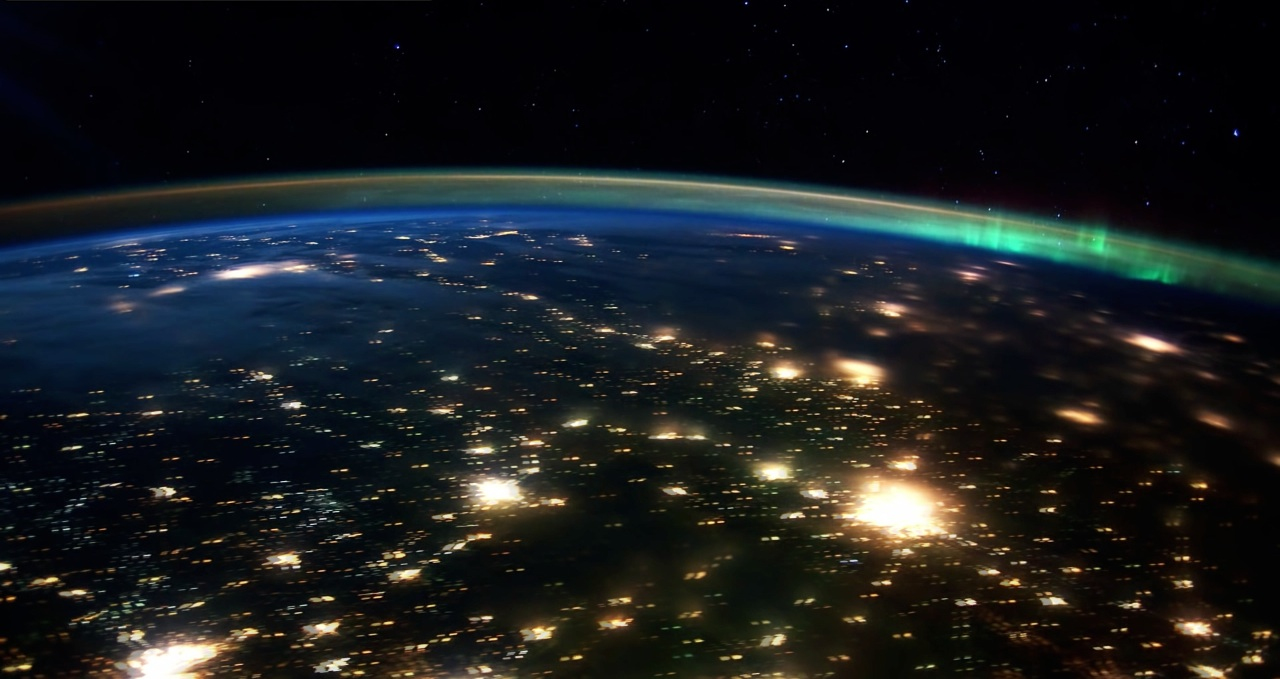
\includegraphics[width=\linewidth]{images/nasaearth.jpg}
              \captionsetup{width=\linewidth}
              \caption[Aurora borealis.]{Aurora borealis one of the most fascinating volumetric phenomenons on earth. This photo also exhibits atmospheric light scattering and city glow at night. Source \cite{AURO}.}\label{fig:AURO}
          \end{figure}
      \end{minipage}
      \hspace{0.05\linewidth}
      \begin{minipage}{0.45\linewidth}
          \begin{figure}[H]
              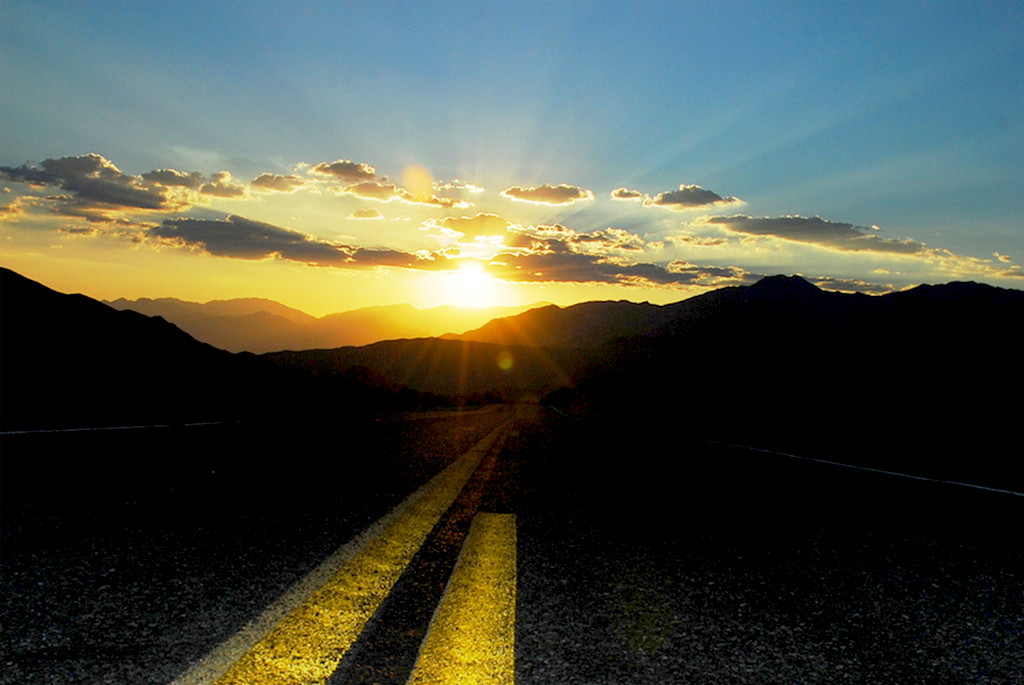
\includegraphics[width=\linewidth]{01_Intro/images/sunset.jpg}
              \captionsetup{width=\linewidth}
              \caption[Crepuscular rays.]{Crepuscular rays also known as good rays are nice example of volumetric shadowing effect, which can be quite believably approximated using only single light scattering. Autor \cite{PETR}.}\label{fig:PETR}
          \end{figure}
      \end{minipage}
  \end{minipage}

\noindent{
\\
\\
In terms of feasible render times only direct illumination component can be computed. This approach can give us satisfying results such as those on the figure (fig \ref{fig:PETR}).  Unfortunately many cool looking effects such as volumetric caustics, which can be seen on the figure (fig \ref{fig:LASER}) are impossible to get using this approach.
\\
\\
}
\myFigure{0.5}{01_Intro/images/laseroptique.jpeg}{Laser optics.}{Laser beam being refracted and reflected multiple times. The beam is visible thanks to interaction with tiny particles floating in the air, which diffract part of the light energy to the camera chip.Source \cite{LOPT}.}{fig:LASER}

\noindent{
This thesis focuses on methods, which can render anything with physical accuracy and without restrictions on the rendered scene. The other very important bonus of these methods is their progressive nature. In the first passes the corse illumination of the scene is computed and it's progressively refined (fig \ref{fig:ITER}). This for example means, that artist defining lighting mood of the visual effect shots can iterate faster. They have got something to show to the director, which results in quick turnarounds and substantial cost and time savings.
}
\\
\myFigure{0.5}{images/temp.jpg}{Progressive rendering.}{Image after first progressive iteration on the left. After ten iterations  in the middle and on the right final quality image after twenty iterations.}{fig:ITER}
\\
\\
Our aim is to implement these progressive Monte Carlo methods in the presence of heterogenous, optically active media and test them on scenes with varying complexity.
\\
\\

%Problem definition tj realistic image synthesis. - done
%
%What is optically active environment and example images. What is challenging in reality immense photon counts, complex light paths and object complexity and dimensionality of the problem. 
%
%Why global illumination - simulace volume caustics (neprime osvetleni muze v osvetlovani hrat i hlavni roli) 
%
%and why progressive methods - artist quick turn arounds with approximated solutions, which show general lighting conditions, quick director approvals. 
%computation is not lost we can continue to render new iterations of the image and increase the fidelity of the image.

% {VULC} vulcano image{images/icevolcano.jpg}
%{LOPT} laser optics {images/laseroptique.jpeg}


\section{Thesis structure}
This Thesis consists of eight main chapters. In the first chapter we have introduced you to the problem. In the second chapter the nifty theoretical details behind realistic image synthesis are exposed and fundamental terms such as BRDF, phase function and rendering equation defined and explained.
\\
\\
The third chapter is an overview of current strategies and algorithms used to visualize the volumetric phenomenons and their pros and cons listed. The fourth chapter leads us to the core of this thesis, the progressive methods of computation the global illumination in the presence of volumetrically active phenomenons.
\\
\\
In the fifth chapter we choose some of the methods mentioned in preceding chapter and further analyze them and propose a way how to and why to use them. In the sixth chapter we present our solution and describe it's internal structure. In the seventh chapter our results and test are shown. And finally eight chapter concludes the information gained and results obtained during this thesis creation.
\\
\\

%\begin{figure}
%   \centering
%   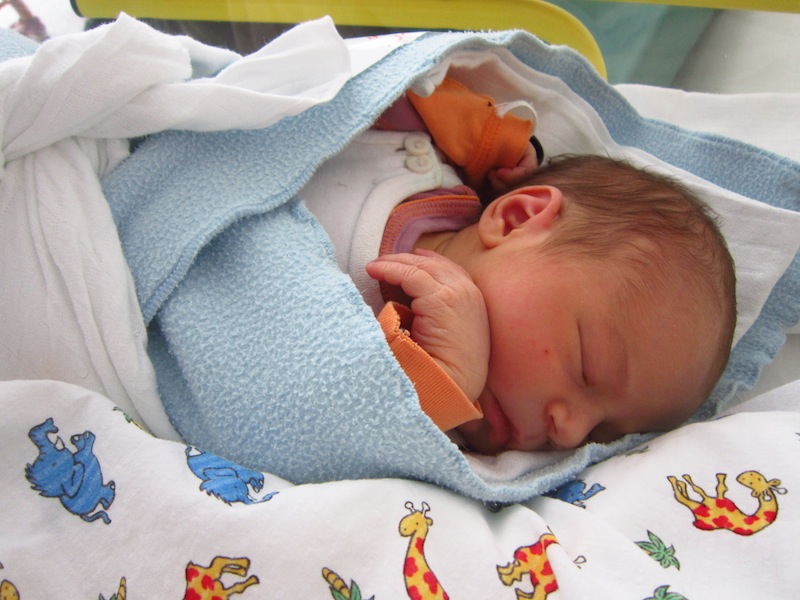
\includegraphics{example.jpg} % requires the graphicx package
%   \caption{example caption}
%   \label{fig:example}
%\end{figure}
%
%   
%Co to je rendering
%Zobrazovaci rovnice distribuce energie v prostoru. 
%
%Co to je raytracing
%paprsek protina geometrii v zakladu 
%
%Jsou stale poupularnejsi progresivni metody renderingu, kdy se obraz pred stale vylepsuje, takze muzem videt nahled velice rychle.
%
%ray tracing se stava poupularnejsi a popularnejsi, mene narocny na nastavovani a fizikalne korektni. Navic sceny jsou slozitejsi a slozitejsi divaci narocnejsi. 
%
%Co to jsou volumetricke efekty a opticky aktivni prostredi
%
%Avsak volumetricke efekty se stale dost casto rasterizujou.
%
%Jak je to náročný a že se stále dost používají aproximační metody (rasterizace, deep shadow maps ) a nemodelují se náročné věci jako radiative transport surface to media volumetric caustics atd. Ani nástroje používané v produkci přímo nepodporuje a nebo jen v podobě náročných fotonových map, je to pomalé , takže artisti nemůžou odladit vse co chteji malo iteraci.



%\section{Podkapitola}
